%% ObjectGraph-Agent -- ICML AUTHOR VERSION (names shown; for supervisors and preprint, NOT for submission), draft v0.3, 23 Nov 2026 (adds Experiment 2, preprint wording)
%% Build: python scripts/make_paper_assets.py && cd paper && latexmk -pdf main.tex
%% Uses the official icml2026.sty/.bst when present in this folder; otherwise a labelled preview style.
\documentclass{article}
\def\icmlshowauthors{}
\usepackage{microtype}
\usepackage[htt]{hyphenat}
\usepackage{graphicx}
\usepackage{booktabs}
\usepackage{float}
\usepackage{amsmath,amssymb,amsthm,mathtools}
\usepackage{xspace}
\usepackage{xcolor}
\usepackage{xcolor}
\definecolor{mydarkblue}{rgb}{0,0.08,0.45}
\usepackage[colorlinks=true,linkcolor=mydarkblue,citecolor=mydarkblue,urlcolor=mydarkblue,filecolor=mydarkblue]{hyperref}
\usepackage{algorithm}
\usepackage{algpseudocode}
\IfFileExists{icml2026.sty}{\usepackage{icml2026}}{\usepackage{icmlpreview}}
% Shared macros for both versions of the paper.
% AUTO-GENERATED by scripts/make_paper_assets.py -- do not edit by hand
\newcommand{\NProjects}{22\xspace}
\newcommand{\NMulti}{11\xspace}
\newcommand{\NSingle}{11\xspace}
\newcommand{\NMultiPython}{2\xspace}
\newcommand{\NMultiCpp}{3\xspace}
\newcommand{\NMultiJava}{5\xspace}
\newcommand{\NMultiJS}{1\xspace}
\newcommand{\CutRedMin}{52\xspace}
\newcommand{\CutRedMax}{97\xspace}
\newcommand{\CutRedMedian}{78\xspace}
\newcommand{\PMax}{0.0105\xspace}
\newcommand{\Draws}{2{,}000\xspace}
\newcommand{\Seed}{20261121\xspace}
\newcommand{\CFErr}{0.4\xspace}
\newcommand{\NBeatGC}{8\xspace}
\newcommand{\NEqGC}{3\xspace}
\newcommand{\NSplitClass}{0\xspace}
\newcommand{\NInfomapSame}{4\xspace}
\newcommand{\NInfomapClose}{9\xspace}
\newcommand{\NInfomapSameK}{4\xspace}
\newcommand{\NLouvainSameK}{6\xspace}
\newcommand{\NLambdaChange}{0\xspace}
\newcommand{\WeightStableAll}{86\xspace}
\newcommand{\WeightStableMulti}{79\xspace}
\newcommand{\WeightARIMulti}{0.92\xspace}
\newcommand{\NClassLevelMulti}{4\xspace}
\newcommand{\KMin}{2\xspace}
\newcommand{\KMax}{7\xspace}
\newcommand{\DutyMin}{4\xspace}
\newcommand{\DutyMax}{50\xspace}
\newcommand{\NRefRan}{9\xspace}
\newcommand{\NRefFull}{6\xspace}
\newcommand{\DevBenchCommit}{bb593c1\xspace}
\newcommand{\PythonVersion}{3.13.18\xspace}
\newcommand{\NumpyVersion}{2.5.3\xspace}

% Results that do not exist yet. Must be empty before submission.
\newcommand{\pending}[1]{\textcolor{red}{[PENDING: #1]}}
% Author details still to be supplied. Must be empty before submission.
\newcommand{\tbd}[1]{\textcolor{blue}{[TO ADD: #1]}}
\theoremstyle{plain}
\newtheorem{proposition}{Proposition}
\newtheorem{assumption}{Assumption}
\theoremstyle{definition}
\newtheorem{definition}{Definition}

\newcommand{\ModelSentence}{\texttt{alibaba/qwen3-coder-30b-a3b} (Qwen3-Coder-30B-A3B-Instruct, an open-weight coding model with a fixed release, accessed through the Vercel AI Gateway)}
\newcommand{\RunHardware}{Agent runs for Python projects were executed on Google Colab (Python 3.13); every scoring run builds a fresh virtual environment. C++ and Java projects are scored in DevBench's container image in GitHub Codespaces.}
\newcommand{\AgentAbstract}{In a pre-registered pilot on 4 Python projects, team designs did not differ in correctness, but where the criterion recommends one agent (3 projects), a single agent was as correct as every split team and used 34--90\% fewer tokens.}
\newcommand{\AgentConclusion}{A pre-registered pilot on 4 Python projects found no correctness difference between team designs, so its go/no-go rules return a provisional NO-GO; but on all 3 projects for which the criterion recommends one agent, following that recommendation was as correct as every split team and cut token use by 34--90\%. The main study will use tasks on which models pass a meaningful share of tests, add a second model, and test H1--H4.}
\newcommand{\ContributionFour}{A pre-registered agent study with four hypotheses, controlled conditions and an equal token budget per run, a zero-cost verification of the agent harness, and a pilot reported in full, including its go/no-go outcome (Section~\ref{sec:agents}).}
\newcommand{\ThreatExtra}{DevBench's tests also check identifiers that are absent from the requirements and the design, which lowers every condition's absolute score; TextCNN is excluded from the pilot because its reference code passes only 5 of 13 tests in the sandbox, as the pre-registered scorer rule requires.}
\newcommand{\PilotDiscussion}{\paragraph{What the pilot shows.} Projects for which the criterion recommends a single agent are where it differs most from graph partitioners. Of the 8 projects with more than one class for which it recommends a single agent, one agent per class splits all 8, Louvain splits 7 and Infomap, the partitioner used by Co-Coder, splits 2 (geotext and particle-swarm-optimization), in both cases into the same teams as one agent per class. Experiment 1b runs exactly these 2 projects, so the single agent is compared with the teams that Infomap, one-agent-per-class and random splitting would use. The pilot was meant to expose problems before the main study, and it did. Its harness checks found and fixed four defects that would otherwise have biased the comparison, and its floor effect shows that, with an open-weight model of this size, DevBench's Python tests are too strict to separate the conditions, because they reward identifiers that the design does not contain. Three changes are therefore proposed for the main study and will be registered before any further run: tasks whose tests call only names that appear in the design, or designs completed with the public interface that the tests call, identically for every condition; a second, stronger model; and token cost and inter-agent messages reported as outcomes alongside tests passed, since the pilot shows that they differ even when correctness does not.}

% generated by scripts/make_exp2_assets.py
\newcommand{\ExpTwoContribution}{A second pre-registered experiment on RealBench \citep{li2026realbench}: a zero-call structural study of all 61 projects, and five team designs compared on 9 real Python projects with their own tests, after a harness check in which every team design reproduces the reference score (Section~\ref{sec:exp2}).}
\newcommand{\ExpTwoAbstract}{A second pre-registered experiment on 9 RealBench projects found no significant quality difference between the criterion's teams and random teams of the same sizes (p = 0.44), but the criterion's teams had the highest mean pass rate (0.21 versus 0.19), used 27\% fewer tokens than random teams, and avoided the collapse of one agent per class, which passed no test on 7 of 9 projects.}
\newcommand{\ExpTwoStructural}{RealBench \citep{li2026realbench} provides 61 Python repositories in four difficulty levels, each with natural-language descriptions, a class diagram generated from the code, a file tree and executable tests. Its diagrams name files without folders and contain no inheritance or composition, so the duty graph reads file paths from the file tree, gives every file an owner (classes, and one unit per file for module-level functions or constants), and uses dependency, import and signature edges. With no model call, the criterion recommends a team for 41 of the 61 projects, and the recommended size grows with difficulty: on average 2.8, 8.2, 4.2 and 18.3 agents for levels 1 to 4 (designs of 3.9, 13.4, 7.7 and 30.4 units). Its team differs from one agent per unit in 39 projects.}
\newcommand{\ExpTwoProtocol}{The tasks were chosen by a rule fixed before any model call: a criterion team of 2 to 6 agents that differs from both one agent per class and Infomap, so that the comparison is informative. Seventeen projects qualify; 8 are unusable because RealBench ships no tests for them or their reference code fails its own tests in the sandbox, which leaves 9. Agents receive the README (when RealBench ships one), the class diagram with its descriptions and the file tree, but never code or tests. Before any model call, the reference code was split according to every team, merged and scored; every team design reproduced the reference score on every task, which rules out losses caused by splitting or merging. This check found and fixed three faults in reading the designs and several in merging; one further merging fault (parenthesized multi-line imports) appeared in the first paid runs and was fixed, and those runs re-merged, before the full run. All fixes are logged. The model is DeepSeek V4.1 Flash (deepseek-v4.1-flash-1017, reasoning off, temperature 0) with three runs per condition and the same token cap as the pilot. The primary hypothesis is that G7 passes more tests than G4 (one-sided Wilcoxon signed-rank test over tasks); G7 against GC and G6 are secondary (Holm-corrected); and the token ratio of G7 to G4 is expected to be at most 1.10. When the first provider's credit ran out after 9 runs, the experiment was moved to a second provider serving the same dated model and rerun in full, as recorded in an amendment.}
\newcommand{\ExpTwoResults}{Six of the 9 tasks have a condition above zero, so the primary hypothesis is testable. It is not supported: G7 wins on 2 tasks, loses on 2 and ties on 5 (p = 0.44; Table~\ref{tab:exp2}). The secondary comparisons point the same way but are not significant either (G7 against GC: 3 wins, 1 loss, Holm-adjusted p = 0.75; against G6: 3 wins, 1 loss, p = 0.75). The criterion's teams nonetheless have the highest mean pass rate (0.21, against 0.19 for random teams, 0.17 for a single agent, 0.15 for Infomap and 0.11 for one agent per class), with their clearest gain on emojichef (0.37 against 0.13 for random teams and 0.12 for a single agent). The cost expectation holds: G7 uses a median 27\% fewer tokens than G4 and 53\% fewer than GC, but 1.6 times as many as a single agent. One agent per class collapses: it passes no test on 7 of the 9 tasks; on crx-analyzer its 22 agents spend about 170k tokens per run and pass nothing, whereas the criterion's 3 agents pass 0.48 of the tests with 18k.}
\newcommand{\ExpTwoDiscussion}{Two results are robust across both experiments. First, the criterion avoids the failure of large teams: splitting by class creates many small agents that each see one class, and the resulting interface mismatches (for example, two agents importing each other's modules) break whole projects. Second, at equal team sizes, grouping duties by the design costs fewer tokens than grouping them at random. Whether that grouping also improves correctness remains open: with 4 non-tied tasks, even 4 wins of 4 would give p = 0.0625, so this experiment could not reach significance, and 3 tasks sat at zero for every condition with this model. A stronger model, which lifts more tasks off the floor, and more tasks are the direct next steps; both will be registered before they run.}
\newcommand{\ExpTwoThreat}{RealBench's diagrams are generated from the code by a static-analysis tool, and its tests may call helpers that the diagram does not list. Only 9 of 17 selected RealBench tasks are usable, and runs at temperature 0 are often identical, which limits the effective sample size.}
\newcommand{\ExpTwoConclusion}{On 9 RealBench projects, the criterion's teams did not significantly beat random teams of the same sizes, but they had the highest mean pass rate, used 27\% fewer tokens than random teams and far fewer than one agent per class, which failed on 7 of 9 projects. The criterion's demonstrated value is therefore efficient, robust team sizing; whether it also improves correctness needs a stronger model and more tasks.}
\newcommand{\ExpTwoFigCaption}{Experiment 2 on RealBench: mean pass rate over three runs per task and condition (top) and median tokens per run (bottom). Cells show the share of the reference code's passing tests that each condition passes.}


\icmltitlerunning{When Should a Software Task Be Split Across LLM Agents?}

\begin{document}
\emergencystretch=1.5em
\twocolumn[
\icmltitle{When Should a Software Task Be Split Across LLM Agents?\\
Cost-Efficient Team Sizing from Domain Models}
\begin{icmlauthorlist}
\icmlauthor{Yashmitha Dilshan}{uow}
\icmlauthor{Achala Aponso}{curtin}
\icmlauthor{Maninda Edirisooriya}{uow}
\end{icmlauthorlist}
\icmlaffiliation{uow}{School of Computing, University of Westminster, London, U.K., in collaboration with the Informatics Institute of Technology, Colombo, Sri Lanka}
\icmlaffiliation{curtin}{School of Electrical Engineering, Computing and Mathematical Sciences, Curtin University, Bentley, WA, Australia}
\icmlcorrespondingauthor{Yashmitha Dilshan}{yashmitha.20211432@iit.ac.lk}
\icmlkeywords{cost efficiency, graph partitioning, large language models, multi-agent systems, software design, software modularization}
\vskip 0.3in
]
\printAffiliationsAndNotice{}

\begin{abstract}
Multi-agent systems built on large language models (LLMs) increasingly develop software, yet team size and the division of work are usually fixed by hand, proposed by a model, or found by costly search, and every extra agent adds tokens and coordination; we ask whether, given the design of the software, the work should be split at all, and into how many agents. We convert a Unified Modeling Language (UML) class diagram into a weighted graph of duties and select, before any code exists, the average-linkage team that maximizes modularization quality minus a per-agent cost, which may be a single agent; we also derive the expected dependency of equal-size random teams in closed form. On all \NProjects DevBench projects, the criterion recommends one agent for \NSingle and teams of \KMin to \KMax agents for \NMulti, with \CutRedMin to \CutRedMax percent less cross-agent dependency than random teams of equal sizes. In pre-registered experiments on RealBench with two model families, the criterion's teams used 27\% and 41\% fewer tokens than random teams of the same sizes, with no significant difference in tests passed, and with the first model avoided the collapse of one agent per class, which passed no test on 7 of 9 projects. Design-time sizing is thus a cheap, reproducible way to reduce the token cost of multi-agent software development and to avoid over-split teams, while a correctness advantage was not found. All code, prompts and cached responses are released.

\end{abstract}

%=====================================================================
\section{Introduction}
\label{sec:intro}

Multi-agent systems built on large language models (LLMs) split one software task among several agents \citep{hong2024metagpt,qian2024chatdev,wu2023autogen}. Someone must decide how many agents to use and what each one owns. Current practice takes one of three routes: fix the roles by hand \citep{hong2024metagpt,qian2024chatdev}, let a model propose a team \citep{ke2025maszero}, or search for or learn a team from scored executions \citep{hu2025adas,zhang2025aflow,zhang2025maas}. None of these routes gives a rule that can be stated, tested and repeated before the work starts.

Peer-reviewed studies make the question pressing. Automatically generated multi-agent systems often trail a single agent at several times the cost \citep{jwalapuram2026illusion}, many reported efficiency gains appear in settings where a single agent or a randomly pruned system already does well \citep{zhang2026rethinking}, and unclear role specification is a major cause of multi-agent failure \citep{cemri2025why}. Recent preprints report consistent trends: multi-agent coordination can hurt on tasks with sequential dependencies \citep{kim2025scaling}, the best number of agents may depend on the task and on the model \citep{li2026scalingbehavior}, and the effective size of a team may grow more slowly than its head count \citep{bertalanic2026ringelmann}. We cite these preprints as motivation, not as established results. Together, this work suggests that the first decision, whether and how to split, deserves its own method and its own controls.

Software engineering has long studied a closely related problem. A good decomposition keeps strongly related responsibilities together and keeps dependencies between parts few \citep{parnas1972criteria,chidamber1994metrics}, and Conway observed that a system's structure mirrors the communication structure of the team that builds it \citep{conway1968committees}. We take this idea literally for LLM agents: if the parts of a design are cohesive and loosely coupled, agents that each own one part should need to communicate less.

\paragraph{This paper.} We study \emph{design-time team sizing}: choosing the number of agents and their responsibilities from a domain model, here a Unified Modeling Language (UML) class diagram, before any code is written. Our contributions are:
\begin{enumerate}
\item A formulation of team sizing as choosing a partition of a design-derived \emph{duty graph}, in which a single agent is a legitimate answer (Section~\ref{sec:problem}).
\item A deterministic criterion based on average-linkage clustering and modularization quality (MQ) with a per-agent cost, together with a closed-form expected cross-agent dependency for random teams of equal sizes and a locality assumption that links that dependency to messages (Section~\ref{sec:method}).
\item A structural study on all \NProjects DevBench projects in four languages, with random, one-agent-per-class, Louvain and Infomap controls and two sensitivity analyses (Section~\ref{sec:structural}).
\item \ContributionFour
\item \ExpTwoContribution
\item A fully deterministic artifact: one command regenerates every number in this paper, and cached model responses allow the agent tables to be rebuilt without calling any model.
\end{enumerate}

\paragraph{Findings in brief.} The evidence supports two claims. First, sizing from the design avoids the failure of over-split teams: one agent per class passed no test on 7 of 9 RealBench projects, whereas the criterion's compact teams had a higher mean pass rate (0.21 against 0.11). Second, at equal team sizes, grouping duties by the design costs fewer tokens than grouping them at random. The evidence does not yet show that the criterion's teams write more correct code than random teams of the same sizes or than a single agent; that claim remains a hypothesis, and Sections~\ref{sec:agents} and~\ref{sec:exp2} report it as not supported in these experiments.

%=====================================================================
\section{Related Work}
\label{sec:related}

\paragraph{Hand-designed and model-designed teams.} MetaGPT and ChatDev encode software-company roles by hand \citep{hong2024metagpt,qian2024chatdev}, and AutoGen provides conversation primitives without a sizing rule \citep{wu2023autogen}. MAS-Zero lets a meta-agent design and refine the system for each problem without a validation set \citep{ke2025maszero}. OOPMAS treats agents as objects and generates query-level workflows \citep{cheng2026oopmas}. Model-driven approaches derive traceable system models from requirements before agents act \citep{wei2026modeldriven}. CodeTeam lets Architect agents propose project-specific plans that fix the number of Developer agents and assign each file an owner, and a CTO agent chooses among them \citep{wang2026codeteam}. These systems decide roles by convention or by model judgment; they do not derive the number of agents from a measurable property of the design or compare that choice with random teams.

\paragraph{Searched, learned and pruned teams.} ADAS and AFlow search over agent programs and workflows using scored executions \citep{hu2025adas,zhang2025aflow}, and MaAS learns a query-dependent distribution over architectures \citep{zhang2025maas}. A second line learns communication topologies over a given pool of agents: G-Designer decodes a task-adaptive topology with a graph auto-encoder \citep{zhang2025gdesigner}, AgentPrune and AgentDropout remove redundant messages and agents \citep{zhang2025agentprune,wang2025agentdropout}, and ARG-Designer generates the collaboration graph autoregressively \citep{li2026argdesigner}. For software development, EvoMAC revises a team of coding agents using test feedback \citep{hu2025evomac}. All of these methods need scored tasks, training runs or test feedback, and most start from a given pool of agents. Our criterion needs none of these and is applied once per design.

\paragraph{How many agents?} In peer-reviewed work, \citet{zhang2026rethinking} recommend evaluating efficiency methods against random and single-agent baselines, and \citet{jwalapuram2026illusion} find that automatically generated multi-agent systems often underperform a single agent. Three recent preprints point in the same direction: \citet{kim2025scaling} model how agent-system performance depends on coordination structure, model capability and task properties and report that coordination can hurt on sequential tasks; \citet{li2026scalingbehavior} report that the best number of agents depends on the task and the model; and \citet{bertalanic2026ringelmann} fit a scaling law for effective team size from small pilot runs on reasoning benchmarks. These studies size teams from executions on reasoning or tool-use tasks; we size them from the structure of a software design, before execution, and adopt their recommended controls.

\paragraph{Closest work: cohesion-aware partitioning of code.} Co-Coder formalizes multi-agent coding as graph partitioning: it builds a dependency graph of repository files by static analysis, isolates hub files, partitions the graph with Infomap community detection \citep{rosvall2008infomap}, and schedules agents along dependencies \citep{yang2026cocoder}. We differ in three ways. First, we work from the \emph{design}, before code exists, so the partition can guide generation rather than reorganize existing code. Second, we choose the team size explicitly, including a single agent, rather than letting a community-detection method set it implicitly. Third, our duties come from the domain model, so each agent action can be traced to a design element. We include Infomap on our own duty graph as a control (condition G6), which separates the partitioning step from the input representation.

\paragraph{Software modularization and design generation.} MQ and the Bunch tool cluster existing source code into modules \citep{mancoridis1998bunch,mitchell2006bunch}, and responsibility-driven design assigns duties to objects \citep{wirfsbrock1989responsibility}. NOMAD generates UML class diagrams from natural-language requirements with a multi-agent pipeline \citep{giannouris2025nomad}, which makes a design-first workflow realistic.

%=====================================================================
\section{Problem Formulation}
\label{sec:problem}

A \emph{domain model} $\mathcal{M}$ is a class diagram with classes, their methods and attributes, and typed relations (association, dependency, aggregation, composition, inheritance and realization).

\begin{definition}[Duty graph]
The duty graph $G(\mathcal{M}) = (V, W)$ has one node, or \emph{duty}, per method of each class; a class without methods contributes one \emph{state duty}. The symmetric weight $W_{uv} \ge 0$ is the sum of four terms: $w_{\text{in}}$ if $u$ and $v$ belong to the same class; $w_{\text{str}}$ if their classes are linked by composition, aggregation, inheritance or realization; $w_{\text{weak}}$ if their classes are linked by association or dependency; and $w_{\text{sig}}$ if the signature of $u$ names the class of $v$, or vice versa. Weights are scaled so that $\max W = 1$.
\end{definition}

A \emph{team} is a partition $\pi = \{C_1, \dots, C_k\}$ of $V$; agent $i$ owns the duties in $C_i$ and the code that implements them. The \emph{cut} of a team,
\begin{equation}
\mathrm{cut}(\pi) = \sum_{i<j} \sum_{u \in C_i,\, v \in C_j} W_{uv},
\label{eq:cut}
\end{equation}
is the total dependency that crosses agent boundaries.

\paragraph{Design-time team sizing.} Given only $\mathcal{M}$, with no code and no scored executions, choose $k$ and $\pi$ so that a team of $k$ agents, each implementing its part, produces correct software at low cost. The choice $k = 1$ must be allowed, because splitting is not always beneficial \citep{jwalapuram2026illusion}.

%=====================================================================
\section{Method}
\label{sec:method}

\subsection{Criterion}
For a team $\pi$ with group sizes $N_i = |C_i|$, let $\mu_i = \sum_{u,v \in C_i} W_{uv}$ (both orders) and $\varepsilon_{ij} = \sum_{u \in C_i, v \in C_j} W_{uv}$. Following \citet{mancoridis1998bunch}, the intra-connectivity (cohesion) of group $i$ is $A_i = \mu_i / N_i^2$, the inter-connectivity (coupling) of groups $i$ and $j$ is $E_{ij} = \varepsilon_{ij} / (N_i N_j)$, and
\begin{equation}
\mathrm{MQ}(\pi) = \frac{1}{k}\sum_{i} A_i \;-\; \binom{k}{2}^{-1}\!\sum_{i<j} E_{ij}, \qquad \mathrm{MQ}(\pi) = A_1 \text{ if } k = 1 .
\label{eq:mq}
\end{equation}
Average-linkage agglomerative clustering on the distance $1 - W$ yields a nested family $\pi_1, \dots, \pi_n$ with exactly $k$ groups at level $k$. We select
\begin{equation}
k^\ast = \arg\max_{k} \; \mathrm{MQ}(\pi_k) - \lambda \frac{k-1}{n-1},
\label{eq:kstar}
\end{equation}
breaking ties towards fewer agents. The penalty $\lambda \ge 0$ charges for each additional agent; $\lambda = 0$ is our pre-registered default and is tuned only on development projects. Algorithm~\ref{alg:criterion} summarizes the procedure. It is deterministic, and its cost is dominated by the clustering step, which is quadratic in the number of duties.

\begin{algorithm}[t]
\caption{Design-time team sizing}
\label{alg:criterion}
\begin{algorithmic}[1]
\Require class diagram $\mathcal{M}$, weights $(w_{\text{in}}, w_{\text{str}}, w_{\text{weak}}, w_{\text{sig}})$, penalty $\lambda$
\State $G \gets$ duty graph of $\mathcal{M}$ \Comment{Definition~1}
\State $\pi_1,\dots,\pi_n \gets$ average-linkage cuts of $1 - W$
\For{$k = 1$ to $n$} \State $s_k \gets \mathrm{MQ}(\pi_k) - \lambda (k-1)/(n-1)$ \EndFor
\State $k^\ast \gets \min \arg\max_k s_k$
\State \Return $k^\ast$ and $\pi_{k^\ast}$ (one agent per group)
\end{algorithmic}
\end{algorithm}

\subsection{The Cost of a Random Team of the Same Sizes}
A fair control keeps the team sizes fixed and changes only \emph{which} duties go together \citep{zhang2026rethinking}. Its expected cut has a closed form.

\begin{proposition}[Expected cut of a random equal-size team]
\label{prop:random}
Let $\sigma$ be a uniformly random assignment of the $n$ duties to groups of fixed sizes $N_1, \dots, N_k$, and let $W_{\text{tot}} = \frac12 \sum_{u,v} W_{uv}$. Then
\begin{equation}
\mathbb{E}[\mathrm{cut}(\sigma)] = W_{\text{tot}} \Bigl(1 - \sum_{i} \frac{N_i (N_i - 1)}{n (n-1)}\Bigr).
\label{eq:randomcut}
\end{equation}
\end{proposition}
\begin{proof}
For any pair $u \neq v$, the probability that both fall in group $i$ is $\frac{N_i}{n}\cdot\frac{N_i - 1}{n-1}$, so they are separated with probability $1 - \sum_i \frac{N_i(N_i-1)}{n(n-1)}$. The result follows from linearity of expectation over edges.
\end{proof}
On all \NMulti multi-agent projects, \eqref{eq:randomcut} matches the mean of \Draws sampled random teams to within \CFErr\% (Appendix~\ref{app:repro}), which also checks the sampler.

\subsection{From Cut Weight to Communication}
\begin{assumption}[Locality]
\label{ass:locality}
Each unit of dependency weight that crosses agent boundaries causes, in expectation, between $a$ and $b$ inter-agent messages ($0 < a \le b$), and dependencies inside one agent cause none.
\end{assumption}
\begin{proposition}
\label{prop:messages}
Under Assumption~\ref{ass:locality}, the expected number of inter-agent messages $M(\pi)$ satisfies $a \cdot \mathrm{cut}(\pi) \le \mathbb{E}[M(\pi)] \le b \cdot \mathrm{cut}(\pi)$. Hence, at equal $k$, the criterion's team is expected to need fewer messages than a random team whenever $b\,\mathrm{cut}(\pi_{k^\ast}) < a\,\mathbb{E}[\mathrm{cut}(\sigma)]$.
\end{proposition}
The proof follows from linearity of expectation. The assumption is strong, and we do not take it for granted: hypothesis H2 tests it directly by correlating cut weight with logged messages per agent pair.

%=====================================================================
\section{Structural Study on DevBench}
\label{sec:structural}

\paragraph{Data.} DevBench \citep{li2024devbench}, also released as DevEval, provides \NProjects software projects in Python, C++, Java and JavaScript, each with a product requirements document, a UML class diagram, an architecture design and executable tests. We use commit \texttt{\DevBenchCommit}. All \NProjects class diagrams parse, and the designs range from \DutyMin to \DutyMax duties.

\paragraph{Pre-set choices.} The weights are $w_{\text{in}}{=}1$, $w_{\text{str}}{=}0.5$, $w_{\text{weak}}{=}0.25$ and $w_{\text{sig}}{=}0.5$, with $\lambda{=}0$ and \Draws random teams per project (seed \Seed). These values were fixed before any agent run. No language model is called in this section. The analysis runs in Python \PythonVersion with NumPy \NumpyVersion.

\paragraph{When to split.} The criterion recommends a single agent for \NSingle projects: ArXiv\_digest (7), Hybrid\_Images (6), area\_calculation (7), chakin (4), geotext (4), hone (20), lice (19), listen-now-frontend (4), logistic\_system (18), particle-swarm-optimization (5), readtime (6)
(duty counts in parentheses). For the remaining \NMulti it recommends teams of \KMin to \KMax agents (Table~\ref{tab:multi}): \NMultiPython Python, \NMultiCpp C++, \NMultiJava Java and \NMultiJS JavaScript projects. Whether the single-agent recommendations are \emph{correct} is an empirical question that the agent study answers (H3).

\begin{table*}[t]
\centering
\caption{Projects for which the criterion recommends a team ($k^\ast > 1$). Cls: classes; $n$: duties; Cut$\downarrow$: reduction in cross-agent dependency against \Draws random teams of the same sizes; $p$: one-sided permutation $p$-value; $\Delta$MQ$_{\text{GC}}$: MQ of the criterion's team minus MQ of one agent per class; ARI$_{\text{IM}}$: adjusted Rand index \citep{hubert1985ari} with the Infomap partition; Stable: weight settings (of 81) that give the same $k^\ast$.}
\label{tab:multi}
\small
\begin{tabular}{@{}llrrrlrrrrr@{}}
\toprule
Project & Lang & Cls & $n$ & $k^\ast$ & Sizes & Cut$\downarrow$\% & $p$ & $\Delta$MQ$_{\text{GC}}$ & ARI$_{\text{IM}}$ & Stable \\
\midrule
graph-cpp & C++ & 7 & 21 & 4 & 8+5+4+4 & 70 & 0.0005 & +0.30 & 1.00 & 57/81 \\
people\_management & C++ & 2 & 14 & 2 & 10+4 & 80 & 0.0010 & +0.00 & 1.00 & 72/81 \\
xlsx2csv & C++ & 4 & 12 & 3 & 5+4+3 & 78 & 0.0005 & +0.09 & 1.00 & 54/81 \\
Actor\_relationship\_game & Java & 7 & 35 & 7 & 7+7+6+6+4+3+2 & 52 & 0.0005 & +0.00 & 0.63 & 63/81 \\
idcenter & Java & 4 & 17 & 3 & 11+3+3 & 97 & 0.0005 & +0.22 & 1.00 & 81/81 \\
image-similarity & Java & 3 & 17 & 2 & 9+8 & 80 & 0.0005 & +0.01 & 0.73 & 54/81 \\
java\_heap & Java & 5 & 36 & 2 & 26+10 & 96 & 0.0005 & +0.30 & 0.97 & 81/81 \\
redis-cache & Java & 10 & 50 & 5 & 26+10+7+6+1 & 92 & 0.0005 & +0.03 & 0.88 & 43/81 \\
login-registration & JS & 4 & 8 & 3 & 3+3+2 & 75 & 0.0105 & +0.15 & 0.79 & 81/81 \\
TextCNN & Py & 5 & 12 & 5 & 4+3+2+2+1 & 65 & 0.0005 & +0.00 & 0.81 & 54/81 \\
stocktrends & Py & 4 & 13 & 3 & 5+4+4 & 74 & 0.0005 & +0.04 & 0.79 & 63/81 \\
\bottomrule
\end{tabular}

\end{table*}

\paragraph{Teams cut far less dependency than random teams.} For all \NMulti projects, the criterion's team has \CutRedMin--\CutRedMax\% less cross-agent dependency than random teams of equal sizes (median \CutRedMedian\%; all $p \le \PMax$; Figure~\ref{fig:cut}). Any method that optimizes a cohesion score should achieve this, so we treat it as a sanity check rather than as evidence that the teams build better software. Performance is the subject of Section~\ref{sec:agents}.

\begin{figure}[t]
\centering
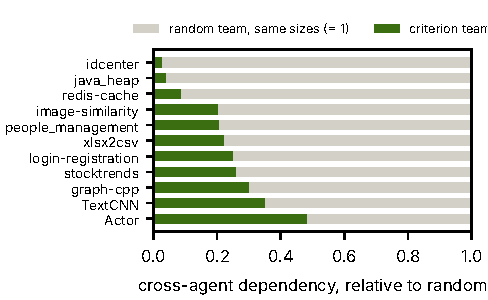
\includegraphics[width=\columnwidth]{figures/cut_vs_random.pdf}
\caption{Cross-agent dependency (cut) of the criterion's team relative to the mean of \Draws random teams with the same group sizes (random $=1$). Lower is better.}
\label{fig:cut}
\end{figure}

\paragraph{Teams group whole classes.} In none of the \NProjects projects does the criterion split a class across agents (\NSplitClass/\NProjects). The duty-level method therefore acts as a principled way of \emph{grouping classes}. Its team scores higher MQ than one agent per class (condition GC) in \NBeatGC of \NMulti projects and coincides with it in \NEqGC. A class-level graph without intra-class weights is too sparse: it recommends a team for only \NClassLevelMulti projects.

\paragraph{Relation to community detection.} Infomap \citep{rosvall2008infomap} produces exactly the same team as our criterion in \NInfomapSame of \NMulti projects and a similar one (adjusted Rand index of at least 0.75) in \NInfomapClose, and Louvain \citep{blondel2008louvain} chooses the same number of agents in \NLouvainSameK. On design graphs, the \emph{partition} is therefore largely determined by the design rather than by the clustering algorithm. What the criterion adds is an explicit, tunable choice of $k$ that includes $k{=}1$, which Infomap and Louvain do not offer. Condition G6 measures whether this matters for agents.

\paragraph{Robustness.} Changing $\lambda \in \{0, 0.05, 0.1, 0.2\}$ changes $k^\ast$ in \NLambdaChange projects. Scaling each of the four weights by $0.5$, $1$ or $1.5$ ($3^4 = 81$ settings) leaves $k^\ast$ unchanged in \WeightStableAll\% of settings on average (\WeightStableMulti\% for multi-agent projects, with a mean adjusted Rand index of \WeightARIMulti against the default team). Figure~\ref{fig:mq} shows representative MQ curves: most have one clear peak, and where a curve has a second peak (redis-cache), the weight grid shows lower stability.

\begin{figure*}[t]
\centering
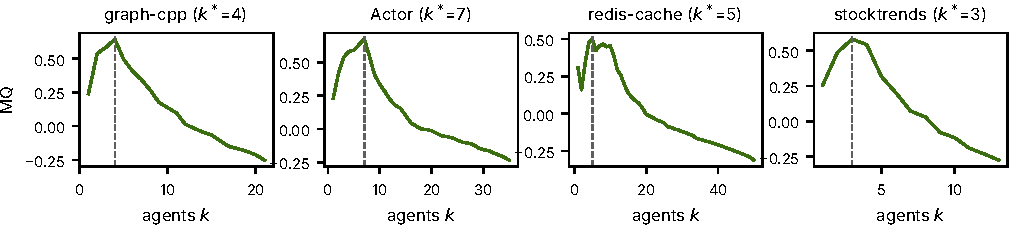
\includegraphics[width=\textwidth]{figures/mq_curves.pdf}
\caption{MQ of the average-linkage team at each size $k$ for four representative projects; the dashed line marks the selected size $k^\ast$.}
\label{fig:mq}
\end{figure*}

%=====================================================================
\section{Agent Study (Pre-Registered)}
\label{sec:agents}

\subsection{Hypotheses}
All thresholds were fixed and recorded in a version-controlled pre-registration file before any agent run.
\begin{itemize}
\item[\textbf{H1}] On projects with $k^\ast > 1$, the criterion's team (G7) passes more reference tests than a random team of equal sizes (G4) and than one agent per class (GC) at an equal token budget (paired Wilcoxon signed-rank test over tasks, Holm-corrected \citep{holm1979simple}, $\alpha = 0.05$).
\item[\textbf{H2}] Across agent pairs, cross-agent dependency weight predicts the number of messages exchanged (Spearman $\rho \ge 0.3$; this tests Assumption~\ref{ass:locality}).
\item[\textbf{H3}] The split or no-split decision ($k^\ast{=}1$ versus $k^\ast{>}1$) agrees with the empirically better choice (best single agent versus best team) more often than chance.
\item[\textbf{H4}] Designs extracted by an LLM from the requirements document give a $k^\ast$ within one of the gold design's in at least 70\% of projects, and H1 still holds with extracted designs.
\end{itemize}

\subsection{Protocol and Conditions}
Every condition uses the same model, decoding settings, prompt templates, orchestrator and token cap; only the division of work changes (Table~\ref{tab:conditions}). Each agent receives the requirements document, the full domain model, the architecture design and the list of duties it owns, each with an identifier. Agents run in the dependency order of the classes they own, and an agent receives the code already written by the agents it depends on; each such hand-over is logged as one message together with its size in tokens. Agents mark every implemented duty with its identifier in a code comment, which gives a traceability score. A deterministic merge step assembles the files, and DevBench's tests score the result in a sandbox from which the reference implementation has been removed.

\begin{table}[t]
\centering
\caption{Conditions. All use the same model, prompts, orchestrator and token cap per run. The pilot runs G2, G4, GC, G6 and G7; the main study adds G1, G3 and G5. When $k^\ast = 1$, G4 uses the group sizes of GC so that splitting can be compared with not splitting.}
\label{tab:conditions}
\small
\begin{tabular}{@{}ll@{}}
\toprule
Condition & Division of work \\
\midrule
G1 & single agent, requirements only \\
G2 & single agent, requirements and design \\
G3 & team size and roles proposed by the LLM \\
G4 & random team, same group sizes as G7 \\
GC & one agent per class \\
G5 & oracle size: best $k$ on development projects \\
G6 & Infomap partition of the same duty graph \\
G7 & criterion team ($k^\ast$, $\pi_{k^\ast}$) \\
\bottomrule
\end{tabular}
\end{table}

\paragraph{Settings.} The pilot uses \ModelSentence{} at temperature 0, at most 8{,}000 output tokens per call, a cap of 200{,}000 tokens per run, three runs per condition with different run identifiers, and the gold design. The main study adds designs extracted from the requirements (H4) and a second model. Every prompt and response is stored with a content hash, so all agent tables can be rebuilt offline. \RunHardware

\paragraph{Scorer validity.} Before scoring any agent, we run DevBench's tests against DevBench's own reference code in our sandbox and against empty code. Of the \NRefRan Python projects we could run, \NRefFull pass every unit and acceptance test (Appendix Table~\ref{tab:ref}); a project is scored only if its reference code passes in full and empty code passes nothing. DevBench's C++ and Java reference code does not build with current compilers (g++ 13, JDK 21), so these projects are scored inside DevBench's own container image. Scorer checks for the C++ and Java pilot projects run in that image and are reported with their results.

\subsection{Results}
\paragraph{Pipeline verification without model calls.} To check that splitting, merging and scoring do not themselves change the outcome, DevBench's reference implementation is cut into the fragments that each agent of each condition would own, merged by the same deterministic merge step as agent output, and scored. Every condition must reach the score of the unsplit reference code, and every condition does (geotext 9/9; hone 12/12; lice 31/31; particle-swarm-optimization 6/6; stocktrends 9/9, for G2, G4, GC, G6 and G7). A smoke run before the pilot exposed four defects in the harness, all fixed before any comparison and applied identically to every condition: a missing package installer on the host, subclasses merged before their base class, traceability markers written by the model without a comment sign, and classes split across agents losing methods in the merge. These changes are listed as deviations in the released pre-registration folder.

\paragraph{Model selection.} The model was chosen before the pilot by a probe that runs only the single-agent condition (G2), so the choice cannot favor any way of splitting. The decision rule was written down before the probe: switch to a larger reasoning model only if it passes at least three more tests in total, and add DevBench's sequence diagram to every agent's input only if it does not lower the score. Neither condition was met (Table~\ref{tab:probe}): the larger model passed the same number of tests at about five times the tokens, and the sequence diagram did not help, so the pilot keeps the cheaper model and the original inputs.



\paragraph{Pilot (Python projects).} Table~\ref{tab:pilot} reports three runs per condition. Correctness did not differ between conditions on any project: on geotext every condition passed the same 0 of 9 tests in every run; on lice every condition passed the same 0 of 31 tests in every run; on particle-swarm-optimization every condition passed the same 4 of 6 tests in every run; on stocktrends every condition passed the same 1 of 9 tests in every run. Scores sit at or near zero on three projects (a floor effect), so the pilot cannot separate the conditions on correctness. Costs did differ (Figure~\ref{fig:pilot}). On every project for which the criterion recommends a single agent (geotext, lice, particle-swarm-optimization), the single agent used fewer tokens than random and one-agent-per-class teams (34--90\% fewer; exact one-sided permutation tests over runs, p = 0.05 for each comparison, the smallest value attainable with three runs per condition) and exchanged no messages; per-project values are in Table~\ref{tab:pilot}. On stocktrends ($k^\ast$ = 3) the criterion team used 14,162 tokens per run against 13,511 for random teams of equal sizes (+5\%, within the pre-registered 10\% margin) and 17,879 for one agent per class and Infomap, which formed the same team (21\% fewer), and exchanged 2 messages against 1 for random teams and 3 for one agent per class. Figure~\ref{fig:teams} shows run 0 of the criterion team and of a random team on stocktrends: the criterion team keeps every class with one agent, so cohesion inside agents is high (0.44--0.75) and coupling between them low (0.00--0.10), whereas the random team spreads classes over agents (cohesion 0.12--0.28, coupling 0.20--0.38); both nevertheless passed the same test, which illustrates that structural quality alone did not translate into correctness on this task. Under the pre-registered rules the pilot is a provisional NO-GO: the criterion team did not pass more tests than random teams on the only scored multi-agent project (a tie, with no strict win); the other rules hold: the criterion team stays within the 10\% token margin of random teams and the single agent is at least as correct as split teams where $k^\ast$ = 1; the decision becomes final once the C++ and Java pilot projects are scored. Experiment 1b, registered before its runs, adds fresh projects for which the criterion recommends one agent: the single agent used fewer tokens than both split teams on every one of the 3 such projects (H3a), and it was at least as correct as the split teams on 1 of the 1 projects on which any condition passed a test (H3b). Inspection of the failing tests shows two causes that affect every condition alike: tests that require identifiers appearing in neither the requirements nor the design (for example, a class constant or a default argument named only in a test), and errors in the model's own code, such as wrong numeric logic or a module that fails at import. The harness itself is not a cause, since the reference code passes every test after the same split and merge. The main study therefore needs tasks on which the model passes a meaningful share of tests; Section~\ref{sec:discussion} discusses this. The whole Python pilot used 408,518 tokens, which cost less than one US dollar with this model.



\begin{figure}[t]\centering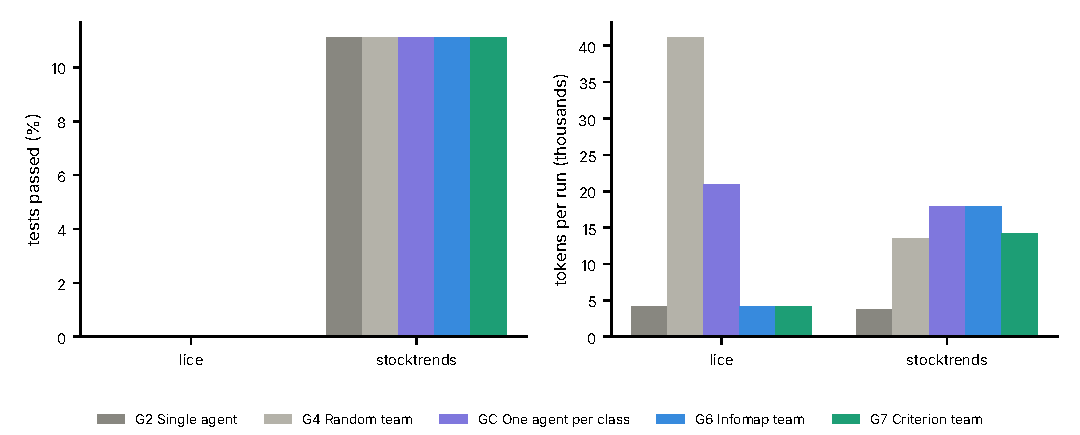
\includegraphics[width=\linewidth]{figures/pilot.pdf}
\caption{Pilot: tests passed (left) and tokens per run (right) for each condition.}\label{fig:pilot}\end{figure}



\textbf{\emph{Main study (planned, pre-registered):}} The confirmatory tests follow the pilot. H1 uses a paired Wilcoxon signed-rank test over tasks with Holm correction and reports bootstrap confidence intervals; H2 correlates cut weight with logged messages per agent pair (Spearman); H3 cross-tabulates the split or no-split decision against the empirically better choice; and H4 repeats H1 with designs extracted from the requirements. The study adds the C++ and Java DevBench projects, further multi-agent tasks to reach the roughly 36 that the power analysis requires, and a second model from a different model family.


%=====================================================================
\section{Experiment 2: RealBench (Pre-Registered)}
\label{sec:exp2}

\paragraph{Setup.} RealBench \citep{li2026realbench} provides 61 Python repositories with class diagrams, file trees and executable tests. Without any model call, the criterion recommends a team for 41 of them, and the recommended size grows with difficulty (Appendix~\ref{app:exp2}). Tasks were chosen by a rule fixed before any model call (a criterion team of 2 to 6 agents that differs from both GC and Infomap); 9 of the 17 qualifying projects have usable tests. Before any model call, the reference code split according to every team, merged and scored reproduced the reference score on every task. The model is deepseek-v4.1-flash-1017 (temperature 0, three runs per condition); the primary test is G7 against G4 (one-sided Wilcoxon over tasks). Full protocol in Appendix~\ref{app:exp2}.

\paragraph{Results.} \ExpTwoResults{} Fig.~\ref{fig:exp2} (Appendix~\ref{app:exp2}) shows every task.

\ExpTwoExploratory

\begin{table}[t]
\centering
\caption{Experiment 2 on RealBench: mean pass rate over three runs (tests passed divided by tests the reference code passes in the same sandbox), with the number of agents in parentheses; tokens are means per run (Mean row: medians). Model: deepseek-v4.1-flash-1017, temperature 0.}
\label{tab:exp2}
\scriptsize
\setlength{\tabcolsep}{2.5pt}
\resizebox{\columnwidth}{!}{\begin{tabular}{@{}llrrrrrr@{}}
\toprule
Task & Lvl & G2 & G4 & GC & G6 & G7 & Tokens G7/G4 \\
\midrule
crules & L1 & 0.80 (1) & 0.80 (2) & 0.80 (6) & 0.80 (6) & 0.80 (2) & 10k / 11k \\
gattino & L1 & 0.00 (1) & 0.00 (3) & 0.00 (6) & 0.00 (6) & 0.00 (3) & 5k / 6k \\
adx-mcp & L2 & 0.07 (1) & 0.01 (2) & 0.00 (4) & 0.00 (4) & 0.00 (2) & 3k / 4k \\
alibaba-dms-mcp & L2 & 0.00 (1) & 0.00 (2) & 0.00 (17) & 0.00 (10) & 0.00 (2) & 15k / 25k \\
crx-analyzer & L2 & 0.32 (1) & 0.48 (3) & 0.00 (22) & 0.22 (4) & 0.48 (3) & 18k / 35k \\
emojichef & L2 & 0.12 (1) & 0.13 (3) & 0.00 (9) & 0.12 (4) & 0.37 (3) & 14k / 20k \\
torchcolor & L2 & 0.00 (1) & 0.00 (4) & 0.00 (19) & 0.00 (7) & 0.00 (4) & 23k / 46k \\
Camera & L3 & 0.13 (1) & 0.13 (4) & 0.00 (5) & 0.00 (5) & 0.04 (4) & 24k / 25k \\
Reconnaissance & L3 & 0.12 (1) & 0.12 (2) & 0.21 (6) & 0.21 (6) & 0.17 (2) & 17k / 22k \\
\midrule
Mean &  & 0.17 & 0.19 & 0.11 & 0.15 & 0.21 & 15k / 22k \\
\bottomrule
\end{tabular}
}
\end{table}




\section{Discussion}\label{sec:discussion}
\label{sec:discussion}

\paragraph{What the structural results do and do not show.} They show that design graphs from a public benchmark have strong cohesive structure, that the criterion finds this structure deterministically and stably, and that it recommends a single agent for half of the projects. They do not show that the recommended teams build better software; only the agent study can show that.

\PilotDiscussion

\paragraph{What Experiment 2 shows.} \ExpTwoDiscussion \ExpTwoHTwoNote

\paragraph{Threats to validity.} \emph{Internal validity:} LLM outputs vary between calls, so every condition runs three times with identical prompts, and identical teams receive identical prompts and cached responses. \emph{Construct validity:} we measure correctness with DevBench's own tests and traceability with duty comments, which may undercount duties implemented without a comment. \emph{External validity:} DevBench projects are small (at most \DutyMax duties), cover four languages and use gold designs written together with the reference code; H4 repeats the main test with designs extracted from requirements, which a real team would have. \emph{Conclusion validity:} DevBench yields only \NMulti multi-agent tasks, below the roughly 36 that our power analysis requires for H1, so the main study will add tasks from benchmarks used in closely related work \citep{yang2026cocoder} and from requirement sets of the kind used by NOMAD \citep{giannouris2025nomad}. \ThreatExtra

\ExpTwoThreat

\paragraph{Weights and contamination.} Edge weights are set by hand. The 81-setting grid shows that $k^\ast$ is stable in most settings but not all, so we report both the default and the full grid and tune nothing on test projects. DevBench is public and may appear in model training data; we compare conditions only with each other, which controls for memorization that affects all conditions equally. DevBench and RealBench are preprints; we use both only as data (designs, requirements and tests), ran their reference code against their own tests before any agent run and used only tasks that pass, and rely on no claim from either paper.

%=====================================================================
\section{Conclusion and Future Work}
\label{sec:conclusion}
Before choosing how to coordinate LLM agents, one must decide whether to split the work at all. We formulated this decision as design-time team sizing, gave a deterministic criterion with a closed-form random baseline, and found on \NProjects DevBench projects that it recommends a single agent for \NSingle and compact teams of \KMin to \KMax agents for the rest, with far less cross-agent dependency than random teams of the same sizes. \AgentConclusion{} \ExpTwoConclusion{} Future work will test the criterion on larger, multi-language benchmarks and with designs that LLMs write from requirements, learn edge weights on development projects instead of setting them by hand, and extend the criterion to teams whose roles change during execution.


\section*{Impact Statement}
This work aims to make LLM-based multi-agent software development cheaper and more predictable by avoiding unnecessary agents, which reduces compute and energy use. Generated code may be incorrect or insecure; in our study all generated code runs only in a sandbox, and the method is intended to support, not replace, human design review.

\bibliography{refs}
\IfFileExists{icml2026.bst}{\bibliographystyle{icml2026}}{\bibliographystyle{plainnat}}

\newpage
\appendix
\onecolumn
\section{Reproducibility}
\label{app:repro}
Every number in Sections~\ref{sec:structural} and \ref{sec:agents} is a macro generated by \texttt{scripts/make\_paper\_assets.py} from \texttt{results/structural.json} and \texttt{results/reference\_tests.json}. The command \texttt{bash reproduce.sh} fetches DevBench at commit \texttt{\DevBenchCommit}, runs the unit tests and regenerates all results, and two runs give byte-identical output. Agent runs store every prompt and response with its hash, so the agent tables can be rebuilt from the cache without calling any model. The pre-registration file and its version-control tag are part of the released code.

\begin{table}[h]
\centering
\caption{DevBench reference code tested against its own tests (Python projects, fresh virtual environment, coverage flags removed).}
\label{tab:ref}
\small
\IfFileExists{generated/table_reference.tex}{\begin{tabular}{@{}lrr@{}}
\toprule
Project & Unit & Acceptance \\
\midrule
ArXiv\_digest & 38/38 & 0/1 \\
Hybrid\_Images & 11/19 & 1/1 \\
TextCNN & \multicolumn{2}{l}{skipped here; 5/13 on Colab} \\
chakin & 0/1 & 0/1 \\
geotext & 4/4 & 5/5 \\
hone & 7/7 & 5/5 \\
particle-swarm-optimization & 5/5 & 1/1 \\
readtime & 8/8 & 4/4 \\
stocktrends & 7/7 & 2/2 \\
lice & 25/25 & 6/6 \\
\bottomrule
\end{tabular}
}{\pending{reference tests}}
\end{table}

\section{Duty-Graph Construction Details}
Mermaid class diagrams are parsed with a tolerant parser that handles class bodies, \texttt{Class : member} lines, generic names such as \texttt{Queue\textasciitilde T\textasciitilde}, cardinalities and labels. Overloaded methods are merged into one duty. Relations to classes that are only mentioned, such as library types, are ignored because no agent implements them, and duplicate relation declarations count once.

\end{document}
